\documentclass{standalone}

\usepackage{tikz}
\usetikzlibrary{positioning, calc, backgrounds, fit, shapes}

% mcs --- memory consistency system. #1: name (an id number) for the node (also used in node text); #2: position
\newcommand{\mcs}[2]{\node (#1) [rectangle split,  rectangle split parts = 3, 
  rectangle split part fill = {lightgray, white, white}, draw, text width = 2.5cm, align = center] at (#2) 
  {Processor $r_{#1}$: \nodepart{two} local memory \nodepart{three} DSM algorithm};}

\begin{document}

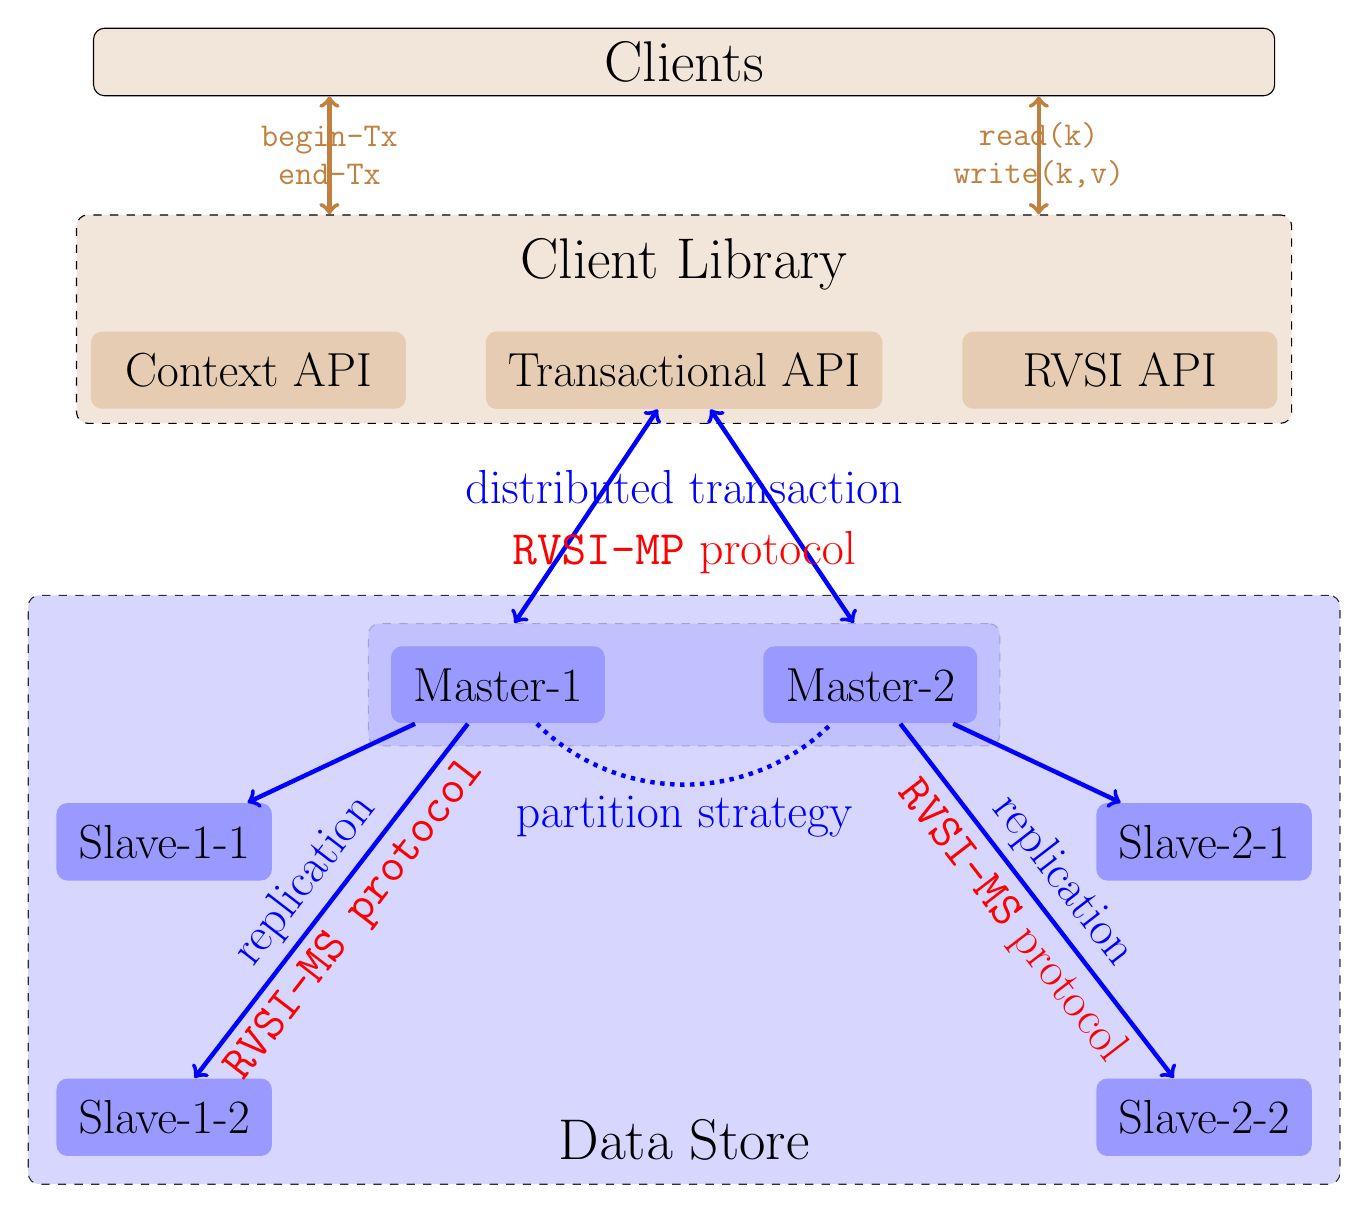
\begin{tikzpicture}[]
  
% client library: transactional api + rvsi api + context api
\begin{scope}[clib/.style = {rectangle, rounded corners, font = \LARGE, fill = brown!40, inner sep = 8pt, minimum width = 4cm}]
  \node (tx-api) [clib] at (0,0) {Transactional API};
  \node (rvsi-api) [clib, right = of tx-api] {RVSI API};
  \node (ctx-api) [clib, left = of tx-api] {Context API};

  % client library text
  \node (client-library-text) [font = \huge, above = 0.40cm of tx-api] {Client Library};

  % surrounding
  \begin{pgfonlayer}{background}
    \node (client-library-surrounding) [rectangle, rounded corners, draw, dashed, fill = brown!20, inner sep = 5pt, fit = (tx-api) 
    (rvsi-api) (ctx-api) (client-library-text)] {};
  \end{pgfonlayer}
\end{scope}

% distributed transaction:
\begin{scope}[master/.style = {rectangle, rounded corners, font = \LARGE, fill = blue!40, inner sep 
  = 8pt}, dist-tx/.style = {<->, outer sep = 3pt, ultra thick, blue}]
  % two masters
  \node (master-left) [master, below left = 3.0cm and 1.0cm of tx-api.south] {Master-1};
  \node (master-right) [master, below right = 3.0cm and 1.0cm of tx-api.south] {Master-2};
  \draw [bend right = 45, dotted, blue, ultra thick] (master-left) to node[font = \LARGE, sloped, below] {partition strategy} (master-right);

  % master surrounding
  \begin{pgfonlayer}{background}
    \node (master-surrounding) [rectangle, rounded corners, draw, dashed, fill = blue!40, inner sep = 8pt, fit = (master-left) (master-right)] {};
  \end{pgfonlayer}

  % distributed transaction
  \draw [dist-tx] (tx-api) to (master-surrounding.160);
  \draw [dist-tx] (tx-api) to (master-surrounding.20);
  \node (dist-tx-text) [font = \LARGE, blue, above = 0.50cm of master-surrounding.north, align = center] {distributed transaction\\\textcolor{red}{\texttt{RVSI-MP} protocol}};
\end{scope}

% replication
\begin{scope}[slave/.style = {rectangle, rounded corners, font = \LARGE, fill = blue!40, inner sep = 
  8pt}, rep/.style = {->, draw, ultra thick, blue}]
  % slaves of master-left
  \node (slave-left-above) [slave, below left = 1.0cm and 1.5cm of master-left] {Slave-1-1};
  \node (slave-left-below) [slave, below = 2.5cm of slave-left-above] {Slave-1-2};
  \draw [rep] (master-left) to (slave-left-above);
  \draw [rep] (master-left) to node[sloped, font = \LARGE, above] {replication} node[sloped, font = \LARGE, below, red] {\texttt{RVSI-MS protocol}} (slave-left-below);
  % slaves of master-right
  \node (slave-right-above) [slave, below right = 1.0cm and 1.5cm of master-right] {Slave-2-1};
  \node (slave-right-below) [slave, below = 2.5cm of slave-right-above] {Slave-2-2};
  \draw [rep] (master-right) to (slave-right-above);
  \draw [rep] (master-right) to node[sloped, font = \LARGE, above] {replication} node[sloped, font = \LARGE, below, red] {\texttt{RVSI-MS} protocol} (slave-right-below);
\end{scope}


% data store surrounding
\begin{pgfonlayer}{background}
  \node (datastore-surrounding) [rectangle, rounded corners, opacity = 0.8, draw, dashed, fill = blue!20, inner sep = 10pt, fit 
  = (master-left) (master-right) (slave-left-above) (slave-left-below) (slave-right-above) 
(slave-right-below) (master-surrounding)] {};
\end{pgfonlayer}

% data store text
\node (datastore-text) [above = 0.20cm of datastore-surrounding.south, font = \huge] {Data Store};

% client
\begin{scope}[access/.style = {<->, brown, ultra thick}]
  \node (client) [above = 1.5cm of client-library-surrounding, draw, fill = brown!20, font = \huge, rectangle, rounded corners, inner sep = 5pt, minimum width = 15.0cm] {Clients};
  \coordinate (client-left) at ($ (client.south west) ! 0.20 ! (client.south east)$);
  \coordinate (client-right) at ($ (client.south west) ! 0.80 ! (client.south east)$);
  \draw [access] (client-left) to node [font = \large, align = center] {\texttt{begin-Tx}\\ 
  \texttt{end-Tx}} (client-left |- client-library-surrounding.north);
  \draw [access] (client-right) to node [font = \large, align = center] {\texttt{read(k)}\\ 
  \texttt{write(k,v)}}(client-right |- client-library-surrounding.north);
\end{scope}

\end{tikzpicture}

\end{document}